\documentclass{article}
\usepackage[utf8]{inputenc}
\usepackage[T1]{fontenc}
\usepackage{graphicx}
\usepackage{hyperref}
\usepackage{geometry}
\geometry{margin=1in}

\title{ENGLAND}
\date{Encyclopaedia Britannica (1771)}

\begin{document}
\maketitle

\section*{Historical source}
\textbf{Entry ID:} \texttt{entry-england-523} \\
\textbf{Volume ID:} 144850375 \\
\textbf{Character Count:} 1599

\subsection*{Extracted Text}
ENGLAND), the founder division of the illand of Great Britain. Including Wales, is at a triangular form, and lies between the 50\textasciicircum{} and 55\textasciicircum{} degrees of north latitudes, extending about 400 miles length from fourth to north, and in the place, it is 300 miles in breadth. It is bounded by Scotland on the north; by the English Channel on the fourth, dividing it from France by the German Sea on the city; and on the well by St George's, or the Irish, Chanel.

At what time to illand of British was people is Where ancestors, nor do we know whether the members or people, northern parts were first inhabited. We have no ac- cousas that can be depended upon before the arrival of Jullou Cedar, and if to certain he found the Southern parts full of people of a very warlike dipofotion. Tehe people, according to Cedar, were a colony of the Guidy, and that opinion is embraced by most of the ancient as well as modern writers. It is slightly founded on the agreement obtered by the Roman between the two nations in their cultures, manners, language, rell- gion, government, way of fighting, \&. The more northern inhabitants, according to Tactics, came from Germany. This he inferen from the make of their limbs, but Cedar family calls them \_Aborigians\_.

England, including the principality of Wales, when inhabited it invaded by the Romans, was divided into a petty by six dir flatter. 1. The Damonnic, called allo Duronomi and green ins- domonic, Danoniis, inhabiting the counties of Cornwall and Devonliire. 2. The Darotriges, who inhabited the track now called \_Derjefihrs.\_ 3. The Belge poffelled Somer-



\section*{Source record}
\begin{itemize}
\item \textbf{Dataset:} \texttt{NationalLibraryOfScotland/encyclopaedia\_britannica\_illustrated}
\item \textbf{Dataset Revision:} \texttt{309f765b1ecc83e0a7f7762e44b4a927a7555443}
\item \textbf{Page ID:} \texttt{britannica:309f765b1ecc83e0a7f7762e44b4a927a7555443:train:523} \\
  \textbf{Filename:} \texttt{page-0523-a583606e375a.jpg} \\
  \textbf{Row Index:} 523 \\
  \textbf{SHA256:} \texttt{a583606e375ad92d...}
\end{itemize}

\begin{figure}[h]
\centering
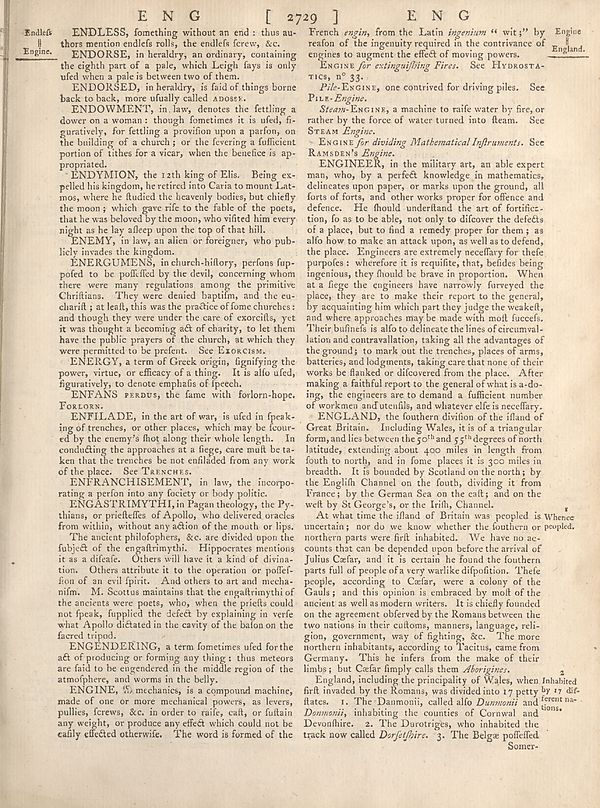
\includegraphics[width=0.85\textwidth]{../scans/page-0523-a583606e375a.jpg}
\caption*{Source scan: \texttt{page-0523-a583606e375a.jpg}}
\end{figure}

\end{document}
